\section{Аналитический раздел}

В данном разделе будет проведен анализ предметной области корпусов текстов, будет формализована задача и данные, описаны пользователи, которые будут взаимодействовать с проектируемым приложением к базе данных, рассмотрены существующие модели данных и будет выбрана одна из моделей для дальнейшей разработки базы данных на ее основе.

\subsection{Анализ предметной области}

Корпусная лингвистика — это раздел компьютерной лингвистики, который занимается разработкой принципов построения и использования корпусов текстов с помощью компьютерных технологий.
Лингвистические корпуса представляют собой структурированные массивы данных, которые используются для изучения языковых единиц в текстах.
В рамках корпуса существует поисковая система, которая позволяет находить необходимые языковые единицы и примеры их употребления благодаря технологии текстовой разметки.
В свою очередь разметка может быть ручной и автоматической.~\cite{butenko2022}

\subsubsection*{Виды корпусов текстов}

В таблице \ref{tab:cc} приведена классификация корпусов текстов по разным признакам.

\begin{table}[H]
    \centering
    \begin{tabular}{|p{5cm}|p{11cm}|}
        \hline
        \textbf{Признак} & \textbf{Типы корпусов} \\ \hline
        Цель & Многоцелевые, специализированные \\ \hline
        Параллельность & Параллельные, сопоставимые \\ \hline
        % Тип языковых данных & Письменные, устные (речевые), смешанные \\ \hline
        % «Литературность» & Литературные, диалектные, разговорные, терминологические, смешанные \\ \hline
        % Жанр & Литературные, фольклорные, драматургические, публицистические \\ \hline
        % Назначение & Исследовательские, иллюстративные \\ \hline
        Динамичность & Динамические (мониторные), статические \\ \hline
        Разметка & Размеченные, неразмеченные \\ \hline
        Характер разметки & Морфологические, синтаксические, семантические, анафорические, просодические и т. д. \\ \hline
        % Доступность & Свободно доступные, коммерческие, закрытые \\ \hline
        Объем текстов & Полнотекстовые, «фрагментнотекстовые» \\ \hline
    \end{tabular}
    \caption{Классификация корпусов~\cite[с. 57]{cl2020}}
    \label{tab:cc}
\end{table}

Корпус технических текстов, для которого будет разрабатываться база данных в настоящей работе, является специализированным, параллельным, многоязыковым, динамическим (будет постоянно пополняться).

\subsubsection*{Параллельные корпусы}

Параллельные корпусы --- корпусы, представляющие собой множество текстов-оригиналов, написанных на каком-либо исходном языке, и текстов --- переводов этих исходных текстов на один или несколько других языков~\cite[с. 61]{cl2020}.

При подготовке параллельных корпусов и разработке программ для их обработки, требуется выровнять тексты --- установить соответствие между фрагментами текста оригинала и текста перевода.
Для решения этой задачи существуют различные методы автоматического выравнивания текстов по предложениям, грамматическим конструкциям, терминам, словам и словосочетаниям.~\cite[с. 61]{cl2020}

Ниже приведен пример выравнивания текстов на уровне предложений.

\begin{table}[H]
    \centering
    \begin{tabular}{|p{1cm}|p{7cm}|p{7cm}|}
        \hline
        1 & THE PLAY — for which Briony had designed the posters, programs and tickets, constructed the sales booth out of a folding screen tipped on its side, and lined the collection box in red crepe paper — was written by her in a two-day tempest of composition, causing her to miss a breakfast and a lunch. & Пьеса, для которой Брайони рисовала афиши, делала программки и билеты, сооружала из ширмы кассовую будку и обклеивала коробку для денежных сборов гофрированной красной бумагой, была написана ею за два дня в порыве вдохновения, заставлявшего ее забывать даже о еде. \\ \hline
        2 & When the preparations were complete, she had nothing to do but contemplate her finished draft and wait for the appearance of her cousins from the distant north. & Когда приготовления закончились, ей не оставалось ничего, кроме как созерцать свое творение и ждать появления кузенов и кузины, которые должны были прибыть с далекого севера. \\ \hline
    \end{tabular}
    \caption{Пример выравнивания текстов на уровне предложений~\cite[с. 62]{cl2020}}
    \label{tab:al}
\end{table}

\subsubsection*{Проблемы определения границ терминов}

При попытке проведения автоматического выравнивания на уровне терминов, возникает ряд проблем.
Среди них выделяют~\cite{butenko2022}:
\begin{itemize}
    \item неправильное определение границ терминов-словосочетаний, состоящих из двух и более слов и составных терминов; 
    \item  распознавание составных терминов и терминов-словосочетаний, состоящих из двух и более слов; в частности, распознавание лексической единицы как части составного термина или как свободной лексической единицы; 
    \item определение лексической единицы как термина в зависимости от контекста и тематики текста, в котором данная лексическая единица употребляется; 
    \item объемные списки терминов-кандидатов, которые необходимо проверять вручную, поскольку частота не является достаточным критерием для оценки того, является ли выделенное слово термином или нет. 
\end{itemize}

Точность определения границ термина при автоматической разметки является одной из основных лингвистических задач, а отсутствие на сегодняшний день информационных систем для автоматической разметки русскоязычных текстов делает актуальным разработку таковой.

% \subsubsection{Тексты и разметки}

\subsubsection*{Типы текстовых разметок}

Существует множество типов текстовых разметок.
Большинство современных корпусов относятся к корпусам морфологического или синтаксического вида~\cite[с. 56]{cl2020}.
% Таким, например, является НКРЯ --- Национальный Корпус Русского Языка~\cite{ruscorpora}.

Далее подробнее будут рассмотрены структурная и семантическая разметки, поскольку они являются основными типами разметки в параллельном корпусе технических текстов.
% TODO: экстралингвистическая разметка cl2020 c. 53

\newpage

\subsubsection*{Структурная разметка}

Структурная разметка предназначена для выделения структурных элементов текста (том, книга, часть, глава, действие, сноска, ремарка, стих, а также: абзац, предложение, словоформа и текстоформа --- таблица, формула и др.)~\cite{lesnikov2019}.
В контексте учебно-научных текстов структурная разметка использована для выделения названия статьи, авторов, оглавления, предисловия, введения и т.д.

На рисунке \ref{fig:ts} представлена структурная схема элементов учебно-научного текста. 

\begin{figure}[H]
	\centering
	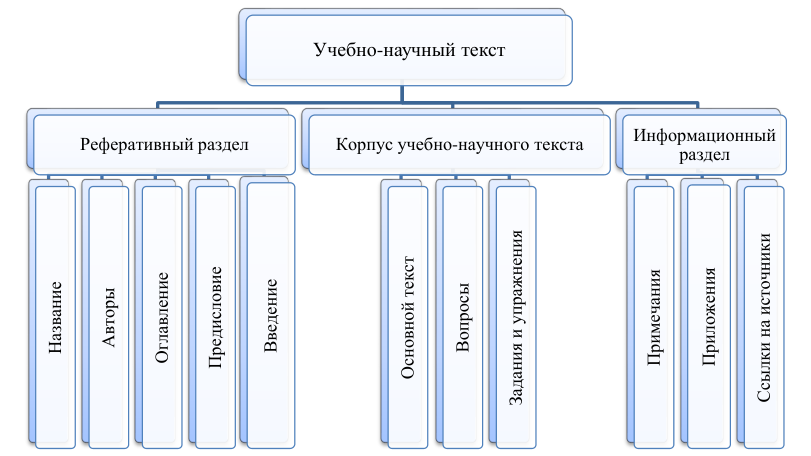
\includegraphics[width=0.9\textwidth]{img/tagging-struct.png}
	\caption{Структурные элементы учебно-научных текстов~\cite{butenko2021}}
	\label{fig:ts}
\end{figure}

\subsubsection*{Семантическая разметка}

Семантическая разметка помогает установить контекст высказывания и устранить двусмысленность. 
Основная цель семантической разметки --- <<формализировать>> значения слов и сделать тексты пригодными для машинной обработки.~\cite{butenko2022-2}

Существует множество видов семантических разметок.
Один из вариантов русской семантической разметки представлен на сайте Центра компьютерных и корпусных языковых исследований Ланкастерского университета~\cite[с. 51]{ucrel, cl2020}:

\begin{table}[H]
    \centering
    \begin{tabular}{|p{5cm}|p{11cm}|}
        \hline
        A & Общие понятия \\ \hline
        A1 & Общие понятия \\ \hline
        A1.1.1 & Обычные действия / Изголовление ч.-л. \\ \hline
        A1.1.1 & Повреждение и разрушение \\ \hline
        A1.2 & Пригодность \\ \hline
        A1.3 & Осторожность \\ \hline
        ... & ............................................................ \\ \hline
        B & Тело человека \\ \hline
        B1 & Анатомия и физиология \\ \hline
        B2 & Здоровье и болезнь \\ \hline
        ... & ............................................................ \\ \hline
        C & Искусства и ремесла \\ \hline
        ... & ............................................................ \\ \hline
    \end{tabular}
    \caption{Русская семантическая разметка~\cite{ucrel}}
    \label{tab:rsm}
\end{table}

В научно-технических текстах для семантической разметки могут использоваться семантические падежи Ч.~Филлмора~\cite{butenko2022-2}.

% \subsubsection*{Структура технических текстов}

\subsection{Существующие решения}

В современном мире существует множество параллельных корпусов (Opus, Linguee, MyMemory, Glosbe, Reverso, TAUS Data Cloud и др.)~\cite{butenko2020-1}, сервисов для автоматического выравнивания текстов (Hunalign, Euclid, Abbyy Aligner, Trados, Winalign, Wordfast tools, Giza++ и др.)~\cite[с. 62]{cl2020}, служб, позволяющих создавать собственные корпусы и производить в них поиск (SketchEngine~\cite{ske}, NoSketchEngine~\cite{noske}); инструментов для автоматического извлечения терминов (TerMine, TermExtraction, Terminology Extraction)~\cite{butenko2022} и прочих инструментов для работы с корпусами текстов (OpenCorpora~\cite{opencorpora}).

Но на данный момент не существует открытых параллельных корпусов технических текстов~\cite{butenko2020-2}.
Также нет открытых информационных систем, позволяющих одновременно производить разметку текста в параллельном корпусе, производить поиск по параллельному корпусу и организовать удобную работу множества разметчиков.

\subsection{Формализация задачи}

В ходе выполнения курсовой работы необходимо спроектировать и разработать базу данных для хранения документов --- технических текстов на разных языках, их разметок, и информации о пользователях базы данных.

Для взаимодействия с базой данных необходимо разработать интерфейс, предоставляющий возможности
\begin{itemize}
    \item добавления новых документов в базу данных,
    \item добавления новых разметок в базу данных,
    \item произведения поиска по текстам и разметкам, хранящимся в базе данных.
\end{itemize}

\subsection{Формализация данных}

Разрабатываемая база данных должна хранить информацию о следующих сущностях:
\begin{itemize}
    \item пользователь;
    \item документ;
    \item метаданные о документе --- автор;
    \item задание на разметку;
    \item структурная разметка;
    \item терминологическая разметка.
\end{itemize}

% \subsection{Сущности базы данных}

% ERD в нотации Чена

На рисунке \ref{fig:chen} представлена диаграмма сущностей разрабатываемой базы данных в нотации Чена.

\begin{figure}[H]
	\centering
	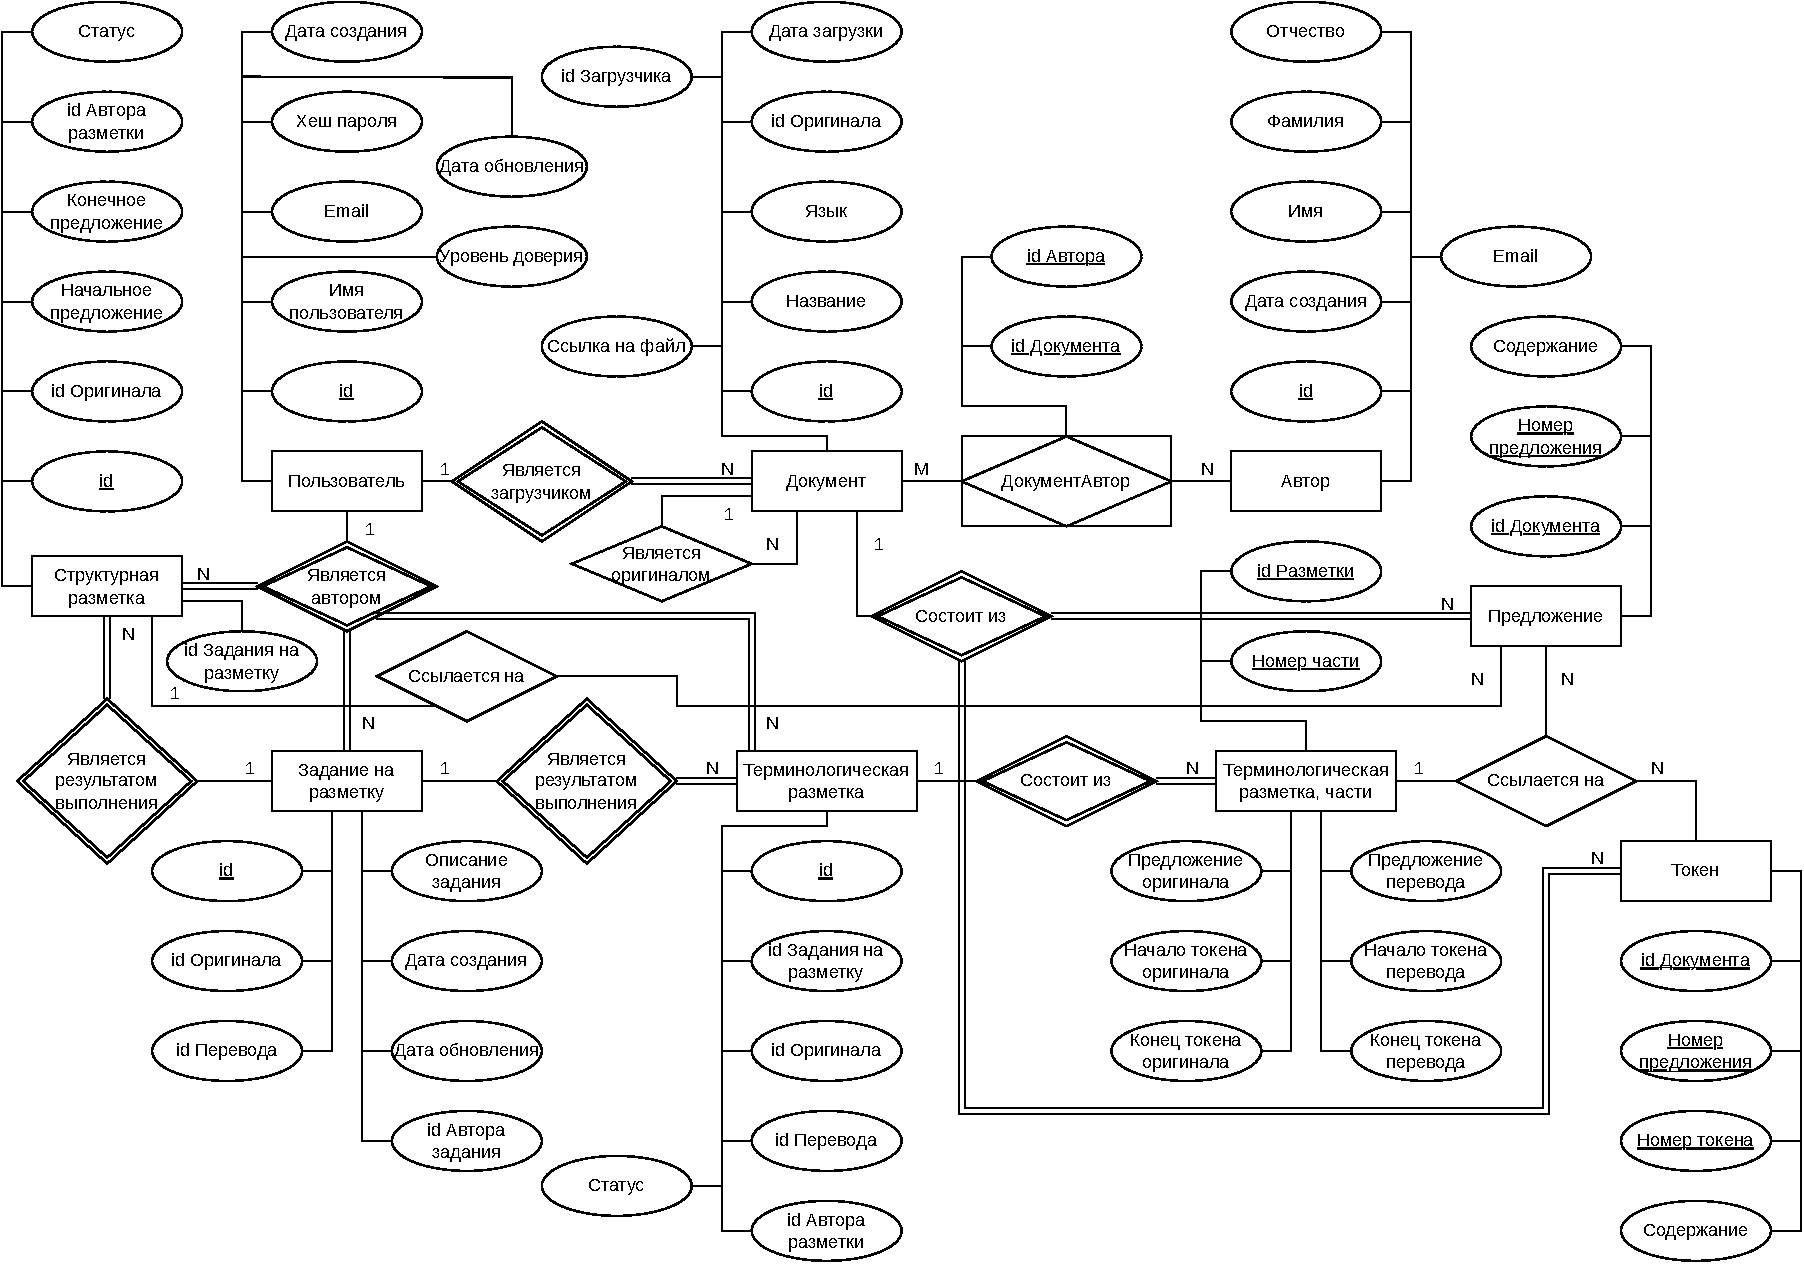
\includegraphics[angle=90, width=\textwidth]{diag/chen-v9.pdf}
	\caption{ER-диаграмма в нотации Чена}
	\label{fig:chen}
\end{figure}

\subsection{Формализация и описание пользователей}

Взаимодействовать с проектируемым приложением к базе данных будут три вида пользователей:
\begin{itemize}
    \item администраторы;
    \item модераторы;
    \item пользователи.
\end{itemize}

Администратор имеет полный доступ к данным: может добавлять, удалять тексты; добавлять, удалять, изменять разметки.

Модераторы производят проверку разметки.

Пользователи имеют возможность осуществлять разметку, которая после своего создания должна пройти модерацию перед публикацией.
Также пользователи могут искать нужные разметку и текст среди уже существующих.

% TODO \cite{butenko2020-2}; 

% \subsection{Сценарии использования}

На рисунке \ref{fig:uc} приведена диаграмма вариантов использования проектируемого приложения к базе данных.

\begin{figure}[H]
	\centering
	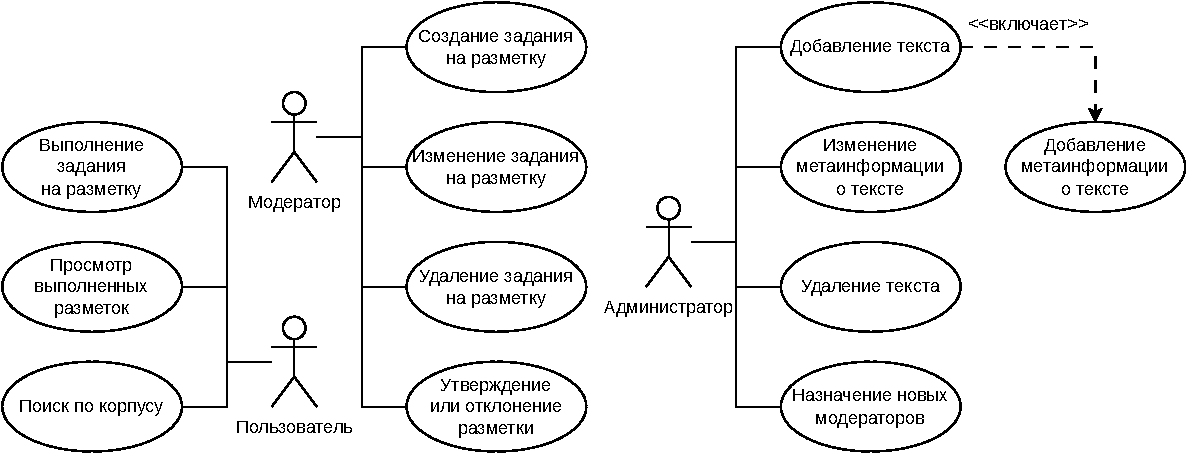
\includegraphics[width=\textwidth]{diag/use-case-v2.pdf}
	\caption{Диаграмма вариантов использования}
	\label{fig:uc}
\end{figure}

\newpage

\subsection{Модели данных}

Модель данных — это абстрактное, самодостаточное, логическое определение объектов, операторов и прочих элементов, в совокупности составляющих абстрактную машину доступа к данным, с которой взаимодействует пользователь.
Упомянутые объекты позволяют моделировать структуру данных, а операторы — поведение данных.~\cite{date}

Дейт выделяет три составляющих моделей данных: структурную, манипуляционную и целостную.~\cite{date-wr}

\subsubsection{Реляционная}

Структурная часть реляционной модели описывает, из каких объектов состоит реляционная модель.
Постулируется, что основной структурой данных, используемой в реляционной модели, являются нормализованные <<n-арные>> отношения.~\cite{date, lecnotes}

В реляционной модели каждый кортеж любого отношения должен отличаться от другого кортежа этого отношения.~\cite{date, lecnotes}

Манипуляционная часть реляционной модели описывает два эквивалентных способа манипулирования реляционными данными --- реляционную алгебру и реляционное исчисление.~\cite{lecnotes}

В целостной части реляционной модели фиксируются два базовых требования целостности, которые должны выполняться для любых отношений в любых реляционных базах данных.
Это целостность сущностей и целостность ссылок.~\cite{lecnotes}

Поддержание целостности сущностей обеспечивается средствами СУБД и осуществляется с помощью двух ограничений:
\begin{enumerate}
    \item при добавлении записей в таблицу проверяется уникальность их первичных ключей,
    \item не позволяется изменение значений атрибутов, входящих в первичный ключ.~\cite{lecnotes}
\end{enumerate}

Требование целостности ссылок состоит в следующем:
Для каждого значения внешнего ключа, появляющегося в дочернем отношении, в родительском отношении должен найтись кортеж с таким же значением первичного ключа.~\cite{lecnotes}

\subsubsection{Инвертированные списки}

Модель инвертированных списков похожа на реляционную, но на более низком уровне абстракции --- хранимые таблицы, а также некоторые пути доступа к этим хранимым таблицам (в частности, некоторые индексы) напрямую доступны пользователю.
Как и реляционная база данных, база данных инвертированных списков содержит множество <<таблиц>> или файлов, и эти <<таблицы>> или файлы разделены на строки (записи) и колонки (поля), как и в реляционном случае.~\cite[с. 388]{date-wr}

Однако, существуют и некоторые значительные различия:
\begin{enumerate}
    \item Строки таблицы инвертированного списка упорядочены в физической последовательности, независимой от индексов.
        Поля внутри строк также упорядочены слева направо.
    \item Определяется общий порядок для базы данных, где строки одной таблицы могут предшествовать строкам другой или чередоваться в определенном порядке.
    \item Можно задать любое количество ключей поиска для таблицы, что позволяет как прямой, так и последовательный доступ на основе этих ключей.
        Индексы не являются прозрачными для пользователя, но их поддержка осуществляется СУБД.
\end{enumerate}

В общем случае операторы манипуляции данными в модели инвертированных списков делятся на две широкие категории:
\begin{enumerate}
    \item Операторы, которые устанавливают адресуемость к какой-либо записи в базе данных (операторы поиска, нахождения или определения местоположения).
    \item Операторы, которые работают с записью по ранее установленному адресу.
\end{enumerate}

Операторы поиска, в свою очередь, делятся на две подкатегории:
\begin{enumerate}[label=\asbuk*)]
    \item Операторы, которые находят запись <<из ниоткуда>> --- то есть операторы прямого поиска.
    \item Операторы, которые находят запись в терминах ее позиции относительно какого-либо ранее установленного адреса --- то есть операторы относительного поиска.~\cite[с. 389]{date-wr}
\end{enumerate}

Модель инвертированных списков не поддерживает общие правила целостности.
Большинство ограничений должны обеспечиваться пользователем, включая ссылочную целостность.~\cite[с. 391]{date-wr}

\subsubsection{Иерархическая}

Иерархическая база данных состоит из упорядоченной коллекции экземпляров одного типа дерева.

Тип дерева включает один корневой тип записи и упорядоченную коллекцию зависимых (нижнего уровня) типов поддеревьев.
Тип поддерева, в свою очередь, также состоит из одного типа записи --- корневого типа поддерева --- и упорядоченной коллекции зависимых типов поддеревьев нижнего уровня.
Таким образом, весь тип дерева представляет собой иерархическую структуру типов записей.~\cite[с. 406]{date-wr}

Основное различие между иерархической и реляционной структурой заключается в следующем: в иерархической базе данных информация, которая в реляционной базе данных представлена внешними ключами, представлена связями <<родитель-ребенок>>.~\cite[с. 408]{date-wr}

Язык манипулирования данными в иерархической базе данных включает операторы для работы с данными в виде деревьев:
\begin{itemize}
    \item Нахождение конкретного дерева в базе данных.
    \item Переход от одного дерева к следующему в иерархической последовательности.
    \item Перемещение от записи к записи внутри дерева по иерархическим путям.
    \item Вставка новой записи в дерево.
    \item Удаление указанной записи.
\end{itemize}

Эти операторы, как правило, работают на уровне записей (манипулируют отдельными записями (или строками) в базе данных, а не группами записей или целыми наборами данных).~\cite[с. 410]{date-wr}

Иерархическая модель автоматически поддерживает ссылочную целостность по правилу: ни один потомок не может существовать без своего родителя.
Если удаляется родитель, система удаляет все поддерево.
Потомок не может быть вставлен без существующего родителя.
Это эквивалентно соблюдению правил внешнего ключа в реляционной модели.~\cite[с. 411]{date-wr}

\subsubsection{Сетевая}

Сетевая база данных состоит из набора записей и связей --- точнее, из любого числа экземпляров нескольких типов записей и связей.
Каждый тип связи включает два типа записей: родительский и дочерний.
Каждый экземпляр связи состоит из одного экземпляра родительского типа записи и упорядоченного набора экземпляров дочернего типа записи.
Для конкретного типа связи L с родительским типом записи P и дочерним типом записи C справедливо следующее:
\begin{itemize}
    \item Каждый экземпляр P является родителем в одном экземпляре L.
    \item Каждый экземпляр C является дочерней записью в не более чем одном экземпляре L.
\end{itemize}

Таким образом, сетевую структуру данных можно рассматривать как расширенную форму иерархической структуры данных.
Основное различие между ними заключается в следующем: в иерархической структуре у дочерней записи есть ровно один родитель; в сетевой структуре у дочерней записи может быть любое количество родителей.~\cite[с. 447]{date-wr}

Язык манипулирования данными в сетевой базе данных состоит из набора операторов для работы с данными, представленными в виде записей и связей.
Примеры таких операторов включают следующее:
\begin{itemize}
    \item Оператор для нахождения конкретной записи по значению какого-либо поля в этой записи;
    \item Оператор для перехода от родителя к его первому ребенку в какой-либо связи;
    \item Оператор для перехода от одного ребенка к следующему в какой-либо связи;
    \item Оператор для перехода от ребенка к родителю в какой-либо связи;
    \item Оператор для создания новой записи;
    \item Оператор для удаления существующей записи;
    \item И так далее.
\end{itemize}

Эти операторы обычно так же, как и в инвертированных списках, и в иерархической модели, работают на уровне записей.

Сетевая модель, как и иерархическая, включает встроенную поддержку ссылочной целостности через связи.
Например, можно задать правило, что дочерняя запись не может быть вставлена без существующего родителя.~\cite[с. 452]{date-wr}

\subsubsection{Постреляционная}

Постреляционная модель расширяет реляционную модель.
Она устраняет ограничение на атомарность данных, позволяя использовать поля с многозначными значениями.
Значения этих полей могут содержать подзначения, и такой набор значений рассматривается как отдельная таблица, встроенная в основную таблицу.~\cite{lecnotes} % XXX actually it's not lecture notes but whatever

% \subsubsection{Выбор модели данных}
\subsection{Выбор модели данных}

Как видно по рисунку \ref{fig:chen}, соблюдения строгой иерархии на диаграмме сущностей разрабатываемой базы данных не наблюдается.
В случае сетевой модели возникают проблемы с выбором <<главного>> элемента, с которого будет осуществляться обход, и с обработкой нескольких путей, ведущих от главного элемента к искомому в случае наличия связи <<многие-ко-многим>>.
Описанная ранее формализация данных лучше всего укладывается в рамки реляционной модели, поэтому в основе разрабатываемой базы данных будет использоваться именно она.
Помимо прочего, у реляционной модели есть еще ряд преимуществ --- современные ее реализации могут автоматически обеспечивать целостность данных и оптимизировать запросы, а также поддерживают транзакционность.

\subsection*{Вывод}

В данном разделе был проведен анализ предметной области корпусов текстов, была формализована задача и данные, описаны пользователи, которые будут взаимодействовать с проектируемым приложением к базе данных, рассмотрены существующие модели данных, и была выбрана реляционная модель.
